%==================///==================///==================///
\begin{frame}{Leveraging the Request Model}
	Requests are key to solve the rebalancing problem
	\begin{columns}
		\begin{column}{0.4\textwidth}
			\begin{itemize}
				\item  Exploiting the deterministic $\lambda$
				\item   Division in regions around depots, i.e. $\mathcal{G}_v = \langle \mathcal{V}'_v, \mathcal{E}'_v\rangle$
				\item 	Rebalancing becomes fundamentally an assignment problem 
			\end{itemize}
		\end{column}
		\begin{column}{0.5\textwidth}
			\begin{figure}
				\centering
				\resizebox{1\textwidth}{!}{
					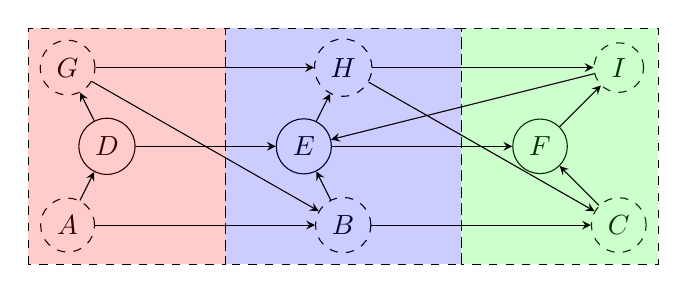
\begin{tikzpicture}[>=stealth]
						
						% Draw rectangle
						%\draw (-1,0) rectangle (8,4);
						
						% Nodes
						\foreach \x/\y/\n in {0/1/A, 3.5/1/B, 7/1/C,  0/3/G, 3.5/3/H, 7/3/I} {
							\node[dashed, circle, draw, fill=white] (\n) at (\x, \y) {$\n$};
						}
						
						\foreach \x/\y/\n in { 0.5/2/D, 3/2/E, 6/2/F} {
							\node[circle, draw, fill=white] (\n) at (\x, \y) {$\n$};
						}
						
						
						% Groups
						\draw[dashed, fill=red, fill opacity=0.2] (-0.5,0.5) rectangle (2,3.5);
						\draw[dashed, fill=blue, fill opacity=0.2] (2,0.5) rectangle (5,3.5);
						\draw[dashed, fill=green, fill opacity=0.2] (5,0.5) rectangle (7.5,3.5);
						
						% Arrows
						\foreach \from/\to in {A/B, B/C, D/E, E/F, G/H, H/I, A/D, B/E, C/F, D/G, E/H, F/I, G/B, H/C, I/E} {
							\draw[->] (\from) -- (\to);
						}
					\end{tikzpicture}
				}
			\end{figure}
			\begin{center}
				$\mathcal{R}_v'= \{ r \in \mathcal{R} : \underline{s_r}' \in \mathcal{V'}_v \} \label{eq:req_per_reg}$
			\end{center}
			
		\end{column}
	\end{columns}
	
\end{frame}

% ==================///==================///==================///
\begin{frame}{Evaluating the MPC performance}
	\begin{columns}
		\begin{column}{0.4\textwidth}
			\begin{table}
				\begin{tabular}{ |l| c|c|c|}
					\cline{2-4}
					\multicolumn{1}{c|}{}&\multicolumn{2}{c|}{No RCS}& RCS\\
					\cline{2-4}
					\multicolumn{1}{c|}{}& 1 &  2&3\\
					\cline{1-4}
					AVs \#& 30&-&-\\
					Horizon (h) & 3 &-& -\\
					Threshold (km/h) & 60&-&-\\
					Requests & 240&-&-\\
					Road (km) & 30&R&-\\
				\end{tabular}
			\end{table}
		\end{column}
		\begin{column}{0.4\textwidth}
			\begin{table}
				\begin{tabular}{ |p{2.9cm}|c|c|c|}
					\cline{2-4}
					\multicolumn{1}{c|}{}&\multicolumn{2}{c|}{No RCS}& RCS\\
					\cline{2-4}
					\multicolumn{1}{c|}{}& 1 &  2&3\\
					\cline{1-4}
					ATT	(\%)		&33&36& 3\\
					ART	(\%)		&17&14 &3\\
					Required AVs			&19&12& 10\\
					Carrying AVs			&13&11&4\\
					Rebalancing AVs			&11&12 &9\\
				\end{tabular}
			\end{table}
		\end{column}
	\end{columns}
\end{frame}
% ==================///==================///==================///


\begin{frame}{System's Performance in a Nutshell}
	\begin{table}[h]
		\centering
		\begin{tabular}{ |p{3.7cm}|c|c|c|c|}
			\cline{2-5}
			\multicolumn{1}{c}{}&\multicolumn{2}{|c|}{w/o Rouing} &\multicolumn{2}{|c|}{w/ Routing}\\
			\cline{2-5}
			\multicolumn{1}{c|}{}& Sim. 1 & Sim. 2 & Sim. 1 & Sim. 2\\
			\hline
			Total Distance (m) &731993& 749006& 806280&874937\\
			Average Distance (m) &30500 & 312089 &33595&36456\\
			Total Time (s) &14640& 14980 &16126&17499\\
			Average Time (s) & 610& 624 &672&729\\
			Unique Road Used &1171&1137 &1193&1206\\
			Request Served (\%)&64 & 63 &81&78\\
		\end{tabular}
	\end{table}
\end{frame}

% ==================///==================///==================///
\begin{frame}{Evaluating the MPC performance}
	\begin{figure}[t]
		\centering
		\resizebox{0.9\textwidth}{!}{
			\begin{tikzpicture}
				\begin{axis}[
					xlabel={Horizon (m)},
					ylabel={$\text{Vehicle Usage}$},
					xmin=0, xmax=20,
					ymin=-2, ymax=25,
					xtick={0,2,4,6,8,10,12,14,16,18,20,22},
					xticklabels={0, 60, 120, 180, 240, 300, 360, 420, 480, 540, 600, 660},
					%xtick={0,2,4,6,8,10,12,14,16,18,20,22},
					%ytick={0,1,2,3,4,5,6,7,8,9,10,11,12,13,14,15,16,17,18,19,20},
					grid=both,
					minor tick num=1,
					width=10cm,
					height=7cm,
					%ymajorgrids=true,
					%grid style=dashed,
					%mark=*,
					%mark options={blue},
					%legend style={at={(0.5,-0.15)},anchor=north,legend columns=-1},
					%legend style={at={(0.5,-0.15)},anchor=north,legend columns=-1, font=\footnotesize},
					legend style={
						at={(1.5,0.5)},
						anchor=east,
						legend columns=1
						legend image post style={scale=0.8} % Adjust the scale as needed
					},
					%legend entries={Plot 1, Plot 2, Plot 3, Plot 4, Plot 5},
					]
					\addplot[viridisbluecolor, mark=*] coordinates {
						(0,0) (1,20) (2,20) (3,20) (4,20) (5,20) (6,20) (7,20) (8,20) (9,20) (10,20) (11,20) (12,20) (13,0) (14,4) (15,3) (16,0) (17,0) (18,3) (19,1) (20,0)(21,0) (22,0)
					};
					\addlegendentry{$i=3, r = 30 \text{ km}$}
					\addplot[viridismagentacolor, mark=+] coordinates {
						(0,0) (1,20) (2,20) (3,20) (4,20) (5,20) (6,20) (7,20) (8,20) (9,20) (10,20) (11,20) (12,20) (13,20) (14,15) (15,13) (16,4) (17,6) (18,3) (19,1) (20,0)(21,0) (22,0)
					};
					\addlegendentry{$i=3, r = 60 \text{ km}$}
					\addplot[viridisorangecolor, mark=o] coordinates {
						(0,0) (1,20) (2,20) (3,20) (4,20) (5,20) (6,20) (7,20) (8,20) (9,20) (10,20) (11,20) (12,20) (13,18) (14,14) (15,5) (16,8) (17,6) (18,8) (19,5) (20,0)(21,0) (22,0)
					};
					\addlegendentry{$i=3, r = 90 \text{ km}$}
					\addplot[viridiscyancolor, mark=x] coordinates {
						(0,0) (1,20) (2,20) (3,20) (4,20) (5,20) (6,20) (7,20) (8,20) (9,20) (10,20) (11,20) (12,20) (13,20) (14,20) (15,20) (16,18) (17,9) (18,7) (19,2) (20,0) (21,0) (22,0)
					};
					\addlegendentry{$i=3, r = 120\text{ km}$}
					\addplot[viridisgreencolor,mark=square] coordinates {
						(0,0) (1,20) (2,20) (3,20) (4,20) (5,20) (6,20) (7,20) (8,20) (9,20) (10,20) (11,20) (12,20) (13,20) (14,20) (15,20) (16,18) (17,9) (18,7) (19,2) (20,0) (21,0) (22,0)
					};
					\addlegendentry{$i=2, r = 150\text{ km}$}
					
					\addplot[viridisbluecolor,mark=square] coordinates {
						(0, 0) (1, 20) (2, 20) (3, 20) (4, 20) (5, 20) (6, 20) (7, 20) (8, 20) (9, 20) (10, 20) (11, 20) (12, 20) (13, 20) (14, 20) (15, 18) (16, 12) (17, 10) (18, 9) (19, 3) (20, 0)
					};
					\addlegendentry{$i=2, r = 180\text{ km}$}
					\addplot[viridismagentacolor,mark=square] coordinates {
						(0, 0) (1, 16) (2, 16) (3, 16) (4, 16) (5, 16) (6, 16) (7, 16) (8, 16) (9, 16) (10, 16) (11, 16) (12, 16) (13, 16) (14, 16) (15, 16) (16, 16) (17, 16) (18, 14) (19, 2) (20, 0)
					};
					\addlegendentry{$i=2, r = 210\text{ km}$}
					\addplot[viridispurplecolor,mark=square] coordinates {
						(0, 0) (1, 20) (2, 20) (3, 20) (4, 20) (5, 20) (6, 20) (7, 20) (8, 20) (9, 20) (10, 20) (11, 20) (12, 20) (13, 20) (14, 20) (15, 20) (16, 19) (17, 14) (18, 8) (19, 2) (20, 0)
					};
					\addlegendentry{$i=4, r = 210\text{ km}$}
				\end{axis}
				
				
				
				
			\end{tikzpicture}
		}
	\end{figure}
\end{frame}
